\documentclass[12pt, titlepage]{article}

\usepackage{fullpage}
\usepackage[round]{natbib}
\usepackage{multirow}
\usepackage{booktabs}
\usepackage{tabularx}
\usepackage{graphicx}
\usepackage{float}
\usepackage{hyperref}
\usepackage{longtable}
\hypersetup{
    colorlinks,
    citecolor=black,
    filecolor=black,
    linkcolor=black,
    urlcolor=blue
}
\usepackage[round]{natbib}

\newcounter{acnum}
\newcommand{\actheacnum}{AC\theacnum}
\newcommand{\acref}[1]{AC\ref{#1}}

\newcounter{ucnum}
\newcommand{\uctheucnum}{UC\theucnum}
\newcommand{\uref}[1]{UC\ref{#1}}

\newcounter{mnum}
\newcommand{\mthemnum}{M\themnum}
\newcommand{\mref}[1]{M\ref{#1}}

\title{SE 3XA3: Module Guide\\SupremeChess}

\author{Team \#2, The Triple Grobs
		\\ Rupinder Nagra (nagrar5)
		\\ Pesara Amarasekera (amarasep)
		\\ Jonathan Cels (celsj)
}

\date{\today}

\begin{document}

\maketitle

\pagenumbering{roman}
\tableofcontents
\listoftables
\listoffigures

\begin{table}[bp]
\caption{\bf Revision History}
\begin{tabularx}{\textwidth}{p{3cm}p{2cm}X}
\toprule {\bf Date} & {\bf Version} & {\bf Notes}\\
\midrule
2021-03-13 & 1.0 & Created document, completed up to anticipated and unlikely changes\\
2021-03-14 & 1.1 & Finished module hierarchy, connections between requirements and design, and started module decomposition\\
2021-03-16 & 1.2 & Finished traceability matrix and the rest of the document\\
2021-03-18 & 1.3 & Minor edits and changes\\
\bottomrule
\end{tabularx}
\end{table}

\newpage

\pagenumbering{arabic}

\section{Introduction}

\subsection{Overview}

The SupremeChess project is the re-implementation of the open-source software application \href{https://github.com/techwithtim/Online-Chess-Game}{``Online-Chess-Game''}, that allows two users to play a game of chess on a server.

\subsection{Context}

This document is the Module Guide (MG), which is created after the Software Requirements Specification (SRS). 

The purpose of the Software Requirements Specification document is to present a description of the software system to be developed, including the functional and non-functional requirements for the project. The following MG has a different purpose, where it is instead providing a modular decomposition of the system, showing the modular structure of the application. The MG also describes how the requirements in the SRS are met with the modular structure that is described.

Along with the MG, it is also necessary to create a Module Interface Specification (MIS) explaining the semantics and syntax of each module. Examples of such semantics and syntax includes the access routines, state variables, inputs/outputs, and exceptions of the modules. This document will further expand on the information provided in the MG.

\subsection{Design Principles}

Information Hiding and Encapsulation are some of the design principles being used to build a modular structure of our application. The project should also assess the software metric of coupling and cohesion. Ideally, the project has high cohesion, and a low degree of coupling.

Information Hiding is the process of hiding the details of an object or function. This process disassociates the calling code from the internal workings of the object or function being called. This makes it possible to change the hidden portions without having to also change the calling code. Encapsulation is a design principle that makes it easier to enforce information hiding. Encapsulation simply hides the states of an object of a class by preventing direct access to it. 

A high cohesion signifies that the methods and data within a module are closely related. Low coupling means that there is a low degree of interdependence between the modules of the system. 

\subsection{Document Structure}
	The document structure is organised as follows:
\begin{itemize}

\item Section 2 lists Anticipated and Unlikely Changes to the system's implementation. This list is used for the Traceability Matrices later in the document.

\item Section 3 presents the Module Hierarchy, listing all the modules and their hierarchy by levels. 

\item Section 4 describes the Connection Between Requirements and Design, which details how the software requirements are related to the modules. 

\item Section 5 describes the Module Decomposition, detailing the module secrets, services, and implementations. 

\item Section 6 provides the Traceability Matrices. The first matrix connects the functional and nonfunctional requirements to the modules. The second matrix connects anticipated changes from Section 2 to the modules.

\item Section 7 presents the Uses Hierarchy diagram for the application. The model shows the uses relations between modules.

\item Section 8 presents the design schedule for the project. A link to the Gantt chart created is provided in this section.

\end{itemize}	


%Start section
\section{Anticipated and Unlikely Changes} \label{SecChange}
\subsection{Anticipated Changes} \label{SecAchange}

\begin{description}
\item[\refstepcounter{acnum} \actheacnum \label{acVerification}:] How user moves are verified.
\item[\refstepcounter{acnum} \actheacnum \label{acInput}:] The format for inputting user moves. Currently click piece and drag to destination, likely to add click piece and click destination.
\item[\refstepcounter{acnum} \actheacnum \label{acBoardState}:] The implementation of the data structure that stores the game board state.
\item[\refstepcounter{acnum} \actheacnum \label{acFontAndPieces}:] User options to change the font and piece models.
\item[\refstepcounter{acnum} \actheacnum \label{acAI}:] AI settings to select and scale difficulty.
\item[\refstepcounter{acnum} \actheacnum \label{acGUI}:] The GUI and interface design.
\item[\refstepcounter{acnum} \actheacnum \label{acTimers}:] User options to play games with different starting timer values.
\end{description}

\subsection{Unlikely Changes} \label{SecUchange}

\begin{description}
\item[\refstepcounter{ucnum} \uctheucnum] Input/output devices to/from the system (Input: Keyboard or Touchscreen, Output: Screen).
\item[\refstepcounter{ucnum} \uctheucnum] The user option to play against another user online.
\item[\refstepcounter{ucnum} \uctheucnum] The interface functionality of the system.
\item[\refstepcounter{ucnum} \uctheucnum] The rules and values related to the game itself.
\item[\refstepcounter{ucnum} \uctheucnum] The purpose of the system to allow users to play a game of chess against an opponent.
\end{description}
%End section

%Start section
\section{Module Hierarchy} \label{SecMH}

\begin{table}[h!]
\centering
\begin{tabular}{p{0.3\textwidth} p{0.6\textwidth}}
\toprule
\textbf{Level 1} & \textbf{Level 2}\\
\midrule

{Hardware-Hiding Module} & ~ \\
\midrule

\multirow{7}{0.3\textwidth}{Behaviour-Hiding Module} 
& Input Module\\
& Output Module\\
& Board Module\\
& Shared Data Module\\
& Piece Module \\
& Game Module\\
\midrule

\multirow{3}{0.3\textwidth}{Software Decision Module}
& App Module\\
& Chat Module\\
& Timer Module\\
& AI Module\\
\bottomrule

\end{tabular}
\caption{Module Hierarchy}
\label{TblMH}
\end{table}
%End section

%Start section
\section{Connection Between Requirements and Design} \label{SecConnection}

The design satisfies the system requirements developed in the SRS. The app module will handle all interactions from the inputs provided by the user and the outputs the program produces. This module will cover all requirements that have a component of the user directly interacting with the system. The AI and chat modules cover the requirements of the AI player, and chat functionality. The board and game modules cover the requirements necessitated (such as checking for legal moves, and end game conditions). The timer module will contain timer classes that will provide the timer information for the game. The look and feel requirements are satisfied by the input and output modules as they define the core areas of user interaction. The usability and humanity requirements are again satisfied by the input and output modules which define the user interaction. Performance requirements are to be satisfied by the combination of all modules, but the key modules that impact performance are software decision hiding modules. The operational and environmental requirements, and the maintainability and support requirements are achieved by all modules. This is because all modules are designed to be operational for the environment (the server and client) and maintained for a set time (end of semester). Security and legal requirements are covered by the entirety of the system. This is because the accessibility of the repository and the JavaScript standard in use affects all modules.

%Start section
\section{Module Decomposition} \label{SecMD}

%Hardware modules
\subsection{Hardware Hiding Module \label{mHH}}

\begin{description}
\item[Secrets:] The design, data structures, and algorithms used in the implementation of the virtual hardware.
\item[Services:] Serves as a virtual hardware used by the rest of the system. This module provides the interface between the hardware and the software. The system can use it to display outputs or to accept inputs.
\item[Implemented By:] OS
\end{description}

%Behaviour modules
\subsection{Behaviour-Hiding Module \label{mBH}}

\begin{description}
\item[Secrets:] The contents of the required behaviour hiding modules.
\item[Services:] These modules describe the application's visible behaviour. They facilitate communication between the Hardware Hiding Module and the Software Decision Modules.
\item[Implemented By:] --
\end{description}

    \subsubsection{Input Module \label{mInput}}
    \begin{description}
    \item[Secrets:] Input data.
    \item[Services:] Allows the user to input game moves into the system.
    \item[Implemented By:] Node.js libraries.
    \end{description}
    
    \subsubsection{Output Module \label{mOutput}} 
    \begin{description}
    \item[Secrets:] Graphics output data.
    \item[Services:] Takes in data on board state, timers, user selection options, and chat messages, and displays it visually.
    \item[Implemented By:] Node.js libraries.
    \end{description}
    
    \subsubsection{Board Module \label{mBoard}}
    \begin{description}
    \item[Secrets:] Board data.
    \item[Services:] Stores and modifies board state information.
    \item[Implemented By:] Node.js libraries.
    \end{description}
    
    \subsubsection{Shared Data Module \label{mSharedData}}
    \begin{description}
    \item[Secrets:] Data.
    \item[Services:] Stores and shares data needed by other modules and between users.
    \item[Implemented By:] JavaScript code.
    \end{description}
    
    \subsubsection{Piece Module \label{mPiece}}
    \begin{description}
    \item[Secrets:] Piece data.
    \item[Services:] Stores piece data and allows for user input to move the piece.
    \item[Implemented By:] Node.js libraries.
    \end{description}
    
    \subsubsection{Game Module \label{mGame}}
    \begin{description}
    \item[Secrets:] Game data.
    \item[Services:] Handles game termination, move handling, and storing previous moves.
    \item[Implemented By:] Node.js libraries.
    \end{description}
    
%Software modules
\subsection{Software Decision Module \label{mSH}}
\begin{description}
\item[Secrets:] Data structures.
\item[Services:] Provides the data structures to store the information from application.
\item[Implemented By:] --
\end{description}

    \subsubsection{App Module \label{mApp}}
    \begin{description}
    \item[Secrets:] Module output data.
    \item[Services:] Compiles and renders all incoming module data.
    \item[Implemented By:] Node.js libraries.
    \end{description}
    
    \subsubsection{Timer Module \label{mTimer}}
    \begin{description}
    \item[Secrets:] Timer data.
    \item[Services:] Stores and processes game timer data.
    \item[Implemented By:] Node.js libraries.
    \end{description}
    
    \subsubsection{Chat Module \label{mChat}}
    \begin{description}
    \item[Secrets:] Chat data.
    \item[Services:] Stores chat messages inputted by players.
    \item[Implemented By:] Node.js libraries.
    \end{description}
    
    \subsubsection{AI Module \label{mAI}}
    \begin{description}
    \item[Secrets:] AI algorithm data.
    \item[Services:] Outputs and performs possible moves by algorithm.
    \item[Implemented By:] Node.js libraries.
    \end{description}
\section{Traceability Matrix} \label{SecTM}

This section shows two traceability matrices: between the modules and the
requirements and between the modules and the anticipated changes.

% the table should use mref, the requirements should be named, use something
% like fref

\begin{center}
    \begin{longtable}{l l l}
        \caption{Trace Between Requirements and Modules} \\
        
        \hline \multicolumn{1}{c}{\textbf{Req.}} & \multicolumn{1}{c}{} & \multicolumn{1}{l}{\textbf{Modules}} \\ \hline 
        \endfirsthead
        
        \multicolumn{1}{c}{\textbf{Req.}} & \multicolumn{1}{c}{} & \multicolumn{1}{l}{\textbf{Modules}} \\ \hline 
        \endhead
        
        \hline \hline
        \endlastfoot
        
        R1 && \mref{mSH}, \mref{mApp}\\
        R2 && \mref{mBH}, \mref{mInput}, \mref{mSH}, \mref{mAI}\\
        R3 && \mref{mBH}, \mref{mGame}\\
        R4 && \mref{mBH}, \mref{mGame}\\
        R5 && \mref{mBH}, \mref{mGame}\\
        R6 && \mref{mBH}, \mref{mGame}, \mref{mSH}, \mref{mApp}\\
        R7 && \mref{mBH}, \mref{mInput}, \mref{mSH}, \mref{mAI}\\
        R8 && \mref{mBH}, \mref{mBoard}, \mref{mGame}, \mref{mSH}, \mref{mApp}\\
        R9 && \mref{mBH}, \mref{mOutput}, \mref{mSharedData}\\
        R10 && \mref{mBH}, \mref{mGame}, \mref{mSH}, \mref{mApp}\\
        R11 && \mref{mBH}, \mref{mGame}, \mref{mSH}, \mref{mApp}\\
        R12 && \mref{mSH}, \mref{mChat}\\
        R13 && \mref{mBH}, \mref{mGame}, \mref{mSH}, \mref{mApp}\\
        R14 && \mref{mBH},  \mref{mInput}, \mref{mSH}, \mref{mAI}\\
        R15 && \mref{mBH}, \mref{mInput} \\
        R16 && \mref{mBH}, \mref{mBoard}, \mref{mGame}\\
        R17 && \mref{mBH}, \mref{mGame}, \mref{mSH}, \mref{mTimer}\\
        R18 && \mref{mBH}, \mref{mPiece}, \mref{mGame}\\
        R19 && \mref{mBH}, \mref{mSharedData}, \mref{mGame}\\
        R20 && \mref{mBH}, \mref{mOutput}, \mref{mPiece}, \mref{mGame}\\
        R21 && \mref{mBH}, \mref{mPiece}, \mref{mGame}\\
        R22 && \mref{mBH}, \mref{mPiece}, \mref{mGame}\\
        R23 && \mref{mBH}, \mref{mPiece}, \mref{mGame}\\
        R24 && \mref{mBH}, \mref{mGame}\\
        R25 && \mref{mBH}, \mref{mGame}, \mref{mSH}, \mref{mTimer}\\
        R26 && \mref{mBH}, \mref{mSharedData}, \mref{mGame}\\
        R27 && \mref{mBH}, \mref{mBoard}, \mref{mGame}\\
        R28 && \mref{mBH}, \mref{mBoard}, \mref{mSharedData}\\
        R29 && \mref{mSH}, \mref{mChat}\\
        R30 && \mref{mSH}, \mref{mChat}\\
        R31 && \mref{mBH}, \mref{mInput}, \mref{mSH}, \mref{mChat}\\
        R32 && \mref{mBH}, \mref{mInput}, \mref{mSH}, \mref{mChat}\\
        R33 && \mref{mBH}, \mref{mInput}, \mref{mSH}, \mref{mChat}\\
        R34 && \mref{mBH}, \mref{mInput}, \mref{mSH}, \mref{mChat}\\
        R35 && \mref{mBH}, \mref{mInput}, \mref{mSH}, \mref{mChat}\\
        R36 && \mref{mBH}, \mref{mInput}, \mref{mSH}, \mref{mChat}\\
        R37 && \mref{mBH}, \mref{mGame}, \mref{mSH}, \mref{mTimer}\\
        R38 && \mref{mBH}, \mref{mGame}, \mref{mSH}, \mref{mTimer}\\
        R39 && \mref{mBH}, \mref{mGame}, \mref{mSH}, \mref{mTimer}\\
        R40 && \mref{mBH}, \mref{mOutput}, \mref{mBoard}, \mref{mGame}\\
        R41 && \mref{mBH}, \mref{mOutput}, \mref{mBoard}, \mref{mGame}\\
        R42 && \mref{mBH}, \mref{mOutput}, \mref{mBoard}, \mref{mGame}\\
        R43 && \mref{mBH}, \mref{mOutput}, \mref{mBoard}, \mref{mGame}\\
        R44 && \mref{mBH}, \mref{mOutput}, \mref{mBoard}, \mref{mGame}\\
        R45 && \mref{mBH}, \mref{mOutput}, \mref{mBoard}, \mref{mGame}\\
        UH2 && \mref{mBH}, \mref{mGame}\\
        UH8 && \mref{mBH}, \mref{mGame}\\
        PR1 && \mref{mBH}, \mref{mInput}, \mref{mOutput}\\
        PR2 && \mref{mBH}, \mref{mInput}, \mref{mOutput}\\
        PR3 && \mref{mBH}, \mref{mInput}, \mref{mOutput}\\
        PR8 && \mref{mBH}, \mref{mInput}, \mref{mOutput}
    \end{longtable}
\end{center}

\begin{center}
    \begin{longtable}{l l l}
        \caption{Trace Between Anticipated Changes and Modules} \\
        
        \hline \multicolumn{1}{c}{\textbf{Req.}} & \multicolumn{1}{c}{} & \multicolumn{1}{l}{\textbf{Modules}} \\ \hline 
        \endfirsthead
        
        \multicolumn{1}{c}{\textbf{Req.}} & \multicolumn{1}{c}{} & \multicolumn{1}{l}{\textbf{Modules}} \\ \hline 
        \endhead
        
        \hline \hline
        \endlastfoot
        
        \acref{acVerification} && \mref{mBH}, \mref{mGame}\\
        \acref{acInput} && \mref{mBH}, \mref{mInput}, \mref{mPiece}\\
        \acref{acBoardState} && \mref{mBH}, \mref{mBoard}, \mref{mPiece}\\
        \acref{acFontAndPieces} && \mref{mBH}, \mref{mOutput}\\
        \acref{acAI} && \mref{mSH}, \mref{mAI}\\
        \acref{acGUI} && \mref{mBH}, \mref{mOutput}\\
        \acref{acTimers} && \mref{mSH}, \mref{mTimer}
    \end{longtable}
\end{center}

\section{Use Hierarchy Between Modules} \label{SecUse}

\begin{figure}[H]
\centering
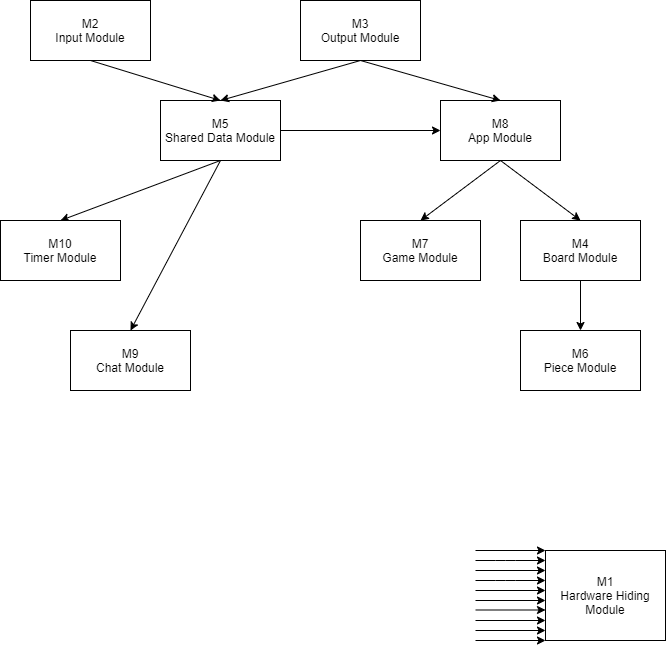
\includegraphics[width=0.9\textwidth]{ModuleHierarchyDiagram.png}
\caption{Use Hierarchy Among Modules}
\label{FigUH}
\end{figure}


\section{Design Schedule}
		
A Gantt chart detailing the project and design schedule can be found at the \href{https://gitlab.cas.mcmaster.ca/celsj/3xa3-group2-chess/-/blob/master/ProjectSchedule/3XA3_ProjectSchedule.pdf}{following link}. 

\bibliographystyle {plainnat}
\bibliography {MG}

\end{document}
